\documentclass[12pt,a4paper]{book}
\newcommand{\niveau}{4\textsuperscript{e}}
\input{../../commun/preambule_commun}

\title{Cours de Mathématiques — Classe de 4\textsuperscript{e}\\[0.4em]\large Année scolaire 2025–2026\\[0.2em]\textcolor{mainBlue}{\normalsize VERSION PROFESSEUR}}
\author{Abdoullatuf Maoulida}
\date{\today}

\begin{document}
% VERSION PROFESSEUR avec toutes les réponses
\VersionCorrige
\maketitle
\tableofcontents
\cleardoublepage

\input{chapitres/seq_01_nombres_relatifs} % Les nombres relatifs
% Chapitre 2 : Théorème de Pythagore et sa réciproque
% Version améliorée conforme à la réforme du collège 2025
% Note: Ce document nécessite les packages tikz, amsmath, amssymb et les environnements personnalisés définis dans le préambule

\chapter{Théorème de Pythagore et sa réciproque}

\section{Introduction}
Le théorème de Pythagore est l'un des théorèmes les plus célèbres et les plus utiles de la géométrie. Il porte le nom de Pythagore, mathématicien et philosophe grec du VI\textsuperscript{e} siècle avant J.-C., bien que cette relation ait été découverte par plusieurs civilisations antérieures.

\subsection*{Un peu d'histoire}
\begin{itemize}
	\item \textbf{Babyloniens (2000 av. J.-C.)} : Utilisaient déjà les triplets pythagoriciens (3, 4, 5) et (5, 12, 13) pour construire des angles droits.
	\item \textbf{Égyptiens} : Les <<tendeurs de corde>> utilisaient une corde à 12 nœuds pour former un triangle 3-4-5 et vérifier les angles droits des pyramides.
	\item \textbf{Pythagore} : A formalisé et démontré le théorème de manière générale.
\end{itemize}

\textbf{Problématique du chapitre :} Comment calculer des longueurs dans un triangle rectangle ? Comment déterminer si un triangle est rectangle ?

\section{Activité — Découvrir l'égalité de Pythagore (GeoGebra)}

\begin{objectifsbox} 
	\begin{itemize}
		\item[\textbullet] Conjecturer la relation entre AB\textsuperscript{2}, BC\textsuperscript{2} et AC\textsuperscript{2}.
		\item[\textbullet] Comprendre le lien entre angle droit et relation entre les carrés des côtés.
	\end{itemize}
\end{objectifsbox}

\subsection*{Manipulation GeoGebra}

\begin{enumerate}
	\item \textbf{Construction du triangle}
	\begin{itemize}
		\item Construire un triangle quelconque $ABC$ et afficher les longueurs $AB$, $BC$, $AC$.
	\end{itemize}
	
	\item \textbf{Préparation du tableur}
	\begin{itemize}
		\item En A1, écrire <<\texttt{AB\string^2 =}>> et, en B1, calculer : \texttt{=(Distance(A,B))\string^2}
		\item En A2 : <<\texttt{BC\string^2 =}>> et en B2 : \texttt{=(Distance(B,C))\string^2}
		\item En A3 : <<\texttt{AC\string^2 =}>> et en B3 : \texttt{=(Distance(A,C))\string^2}
		\item En A4 : <<\texttt{AB\string^2 + BC\string^2 =}>> et en B4 : \texttt{=B1+B2}
	\end{itemize}
	
	\item \textbf{Expérimentation}\\
	Déplacer $A$, $B$ ou $C$ pour rendre le triangle rectangle en $B$ et compléter le tableau :
	
	\begin{center}
		\begin{tabular}{|c|c|c|c|c|l|}
			\hline
			\textbf{Triangle} & \textbf{AB²} & \textbf{BC²} & \textbf{AC²} & \textbf{AB² + BC²} & \textbf{Observation} \\
			\hline
			Rectangle 1 & & & & & \\
			\hline
			Rectangle 2 & & & & & \\
			\hline
			Non rectangle & & & & & \\
			\hline
		\end{tabular}
	\end{center}
	
	\item \textbf{Conclusion :} Que remarquez-vous quand le triangle est rectangle en $B$ ?\\
	..........................................................................................................................................................\\
	..........................................................................................................................................................
\end{enumerate}

\section{Définitions et vocabulaire}

\begin{definitionbox}[Vocabulaire du triangle rectangle]
	\begin{minipage}[t]{0.55\linewidth}\vspace{0pt}
		Un triangle ayant un angle droit est un triangle rectangle.  
		Les deux côtés perpendiculaires d'un triangle rectangle sont les \textbf{côtés de l'angle droit}.  
		Le côté restant est l'\textbf{hypoténuse} du triangle rectangle.  
		C'est le \textbf{côté opposé} à l'angle droit.
	\end{minipage}\hspace{8mm}
	\begin{minipage}[t]{0.4\linewidth}\vspace{0pt}\centering
		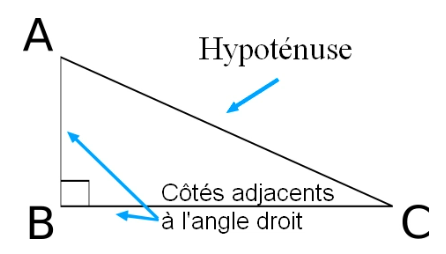
\includegraphics[width=\linewidth]{../../assets/images/4e/seq_02_pythagore/vocabulaire_triangle_rectangle}
	\end{minipage}
\end{definitionbox}

\begin{proprietebox}[Hypoténuse]
	Si un triangle est rectangle alors son plus grand côté est l'hypoténuse.
\end{proprietebox}

\begin{remarkbox}[Piège fréquent]
	L'hypoténuse n'est PAS un des côtés de l'angle droit ! C'est le côté OPPOSÉ à l'angle droit.
\end{remarkbox}

\textbf{Auto-test rapide :} Dans un triangle $DEF$ rectangle en $E$ :
\begin{itemize}
	\item Les côtés de l'angle droit sont : \trous{2cm} et \trous{2cm}
	\item L'hypoténuse est : \trous{2cm}
\end{itemize}

\section{Le théorème de Pythagore}

\subsection{Énoncé du théorème}

\begin{theoremebox}[Théorème de Pythagore]
	Dans un triangle rectangle, le carré de la longueur de l'hypoténuse est égal à la somme des carrés des longueurs des deux autres côtés.
	
	\textbf{Formulation mathématique :}\\
	Si $RKA$ est un triangle rectangle en $K$, alors : $RA^2 = RK^2 + KA^2$ (\textbf{Égalité de Pythagore})
	
	\begin{center}
		% Figure simple du triangle rectangle sans TikZ complexe
		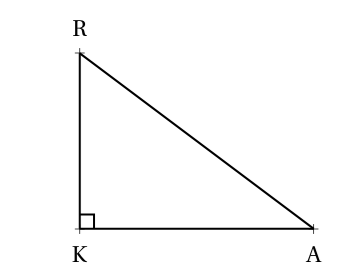
\includegraphics[width=0.3\textwidth]{../../assets/images/4e/seq_02_pythagore/triangle_RKA_rectangle_en_K}
	\end{center}
\end{theoremebox}

\subsection{Démonstration du théorème par la méthode des aires}

Considérons un carré de côté $(a + b)$ contenant quatre triangles rectangles identiques de côtés $a$, $b$ et d'hypoténuse $c$.

\begin{figure}[h]
	\centering
	\begin{minipage}{0.45\textwidth}
		\centering
		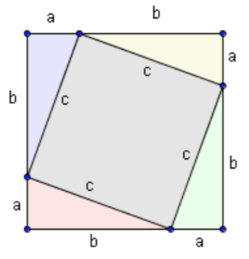
\includegraphics[width=0.8\textwidth]{../../assets/images/4e/seq_02_pythagore/fig_demo_pythagore_config_1}
		\caption{Configuration 1}
	\end{minipage}
	\hfill
	\begin{minipage}{0.45\textwidth}
		\centering
		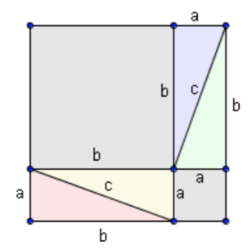
\includegraphics[width=0.8\textwidth]{../../assets/images/4e/seq_02_pythagore/fig_demo_pythagore_config_2.png}
		\caption{Configuration 2}
	\end{minipage}
\end{figure}

\begin{demobox}[Démonstration complète]
	\textbf{Configuration 1 :}
	\begin{itemize}
		\item Aire totale = $(a+b)^2$
		\item Aire = 4 triangles + carré central de côté $c$
		%\item Aire = $4 \times \frac{ab}{2} + c^2 = 2ab + c^2$
		\item Aire = .............................................+.....................................
		
	\end{itemize}
	
	\textbf{Configuration 2 :}
	\begin{itemize}
		\item Aire totale = $(a+b)^2$
		\item Aire = 4 triangles + carré de côté $a$ + carré de côté $b$
		%\item Aire = $4 \times \frac{ab}{2} + a^2 + b^2 = 2ab + a^2 + b^2$
		\item Aire = .......................................+.........................................+...................................
	\end{itemize}
	
	\textbf{Conclusion :} Les deux aires sont égales, donc :
	$$2ab + c^2 = 2ab + a^2 + b^2$$
	$$\boxed{c^2 = a^2 + b^2}$$
\end{demobox}

\subsection{Comprendre la racine carrée}

\begin{definitionbox}[La racine carrée]
	Pour tout nombre positif $a$, il existe un unique nombre \textbf{positif} dont le carré vaut exactement le nombre $a$.
	
	Ce nombre s'appelle la \textbf{racine carrée} de $a$ et se note $\sqrt{a}$.
	
	Par définition : $(\sqrt{a})^2 = \sqrt{a} \times \sqrt{a} = a$
	
	\textbf{Intuitivement :} La racine carrée <<défait>> ce que le carré a fait.
\end{definitionbox}

\begin{examplebox}[Carrés parfaits à connaître par cœur]
	\begin{center}
		\begin{tabular}{|c|c|c|c|c|c|c|c|c|c|c|c|c|c|c|c|}
			\hline
			$n$ & 0 & 1 & 2 & 3 & 4 & 5 & 6 & 7 & 8 & 9 & 10 & 11 & 12 & 13 & 15 \\
			\hline
			$n^2$ & 0 & 1 & 4 & 9 & 16 & 25 & 36 & 49 & 64 & 81 & 100 & 121 & 144 & 169 & 225 \\
			\hline
		\end{tabular}
	\end{center}
	
	\textbf{Astuces de mémorisation :}
	\begin{itemize}
		\item $\sqrt{144} = ......$ 
		\item $\sqrt{225} = ......$
		\item $\sqrt{169} = ......$
	\end{itemize}
\end{examplebox}

\section{Applications du théorème de Pythagore}

\subsection{Calculer la longueur de l'hypoténuse}

\begin{methodebox}[Méthode pas à pas]
	Pour calculer la longueur de l'hypoténuse d'un triangle rectangle :
	\begin{enumerate}
		\item Identifier que le triangle est rectangle
		\item Repérer l'hypoténuse (côté opposé à l'angle droit)
		\item Écrire l'égalité de Pythagore
		\item Calculer les carrés des côtés de l'angle droit
		\item Additionner ces carrés
		\item Prendre la racine carrée du résultat
	\end{enumerate}
\end{methodebox}

\begin{examplebox}[Exemple guidé]
	On étudie le triangle $RAK$ rectangle en $K$ tel que $KR = 4,95$ cm et $KA = 6,6$ cm. Calculons la mesure du côté $[AR]$.
	
	\noindent
	\begin{minipage}[c]{0.60\textwidth}
		\textbf{Solution complète :}
		
		Le triangle $RAK$ est rectangle en $K$.
		
		L'hypoténuse est $[AR]$ (côté opposé à l'angle droit $K$).
		
		D'après le théorème de Pythagore :
		\begin{align*}
			AR^2 &= KR^2 + KA^2\\
			AR^2 &= 4,95^2 + 6,6^2\\
			AR^2 &= 24,5025 + 43,56\\
			AR^2 &= 68,0625\\
			AR &= \sqrt{68,0625}\\
			AR &= 8,25 \text{ cm}
		\end{align*}
	\end{minipage}
	\hfill
	\begin{minipage}[c]{0.35\textwidth}
		\centering
		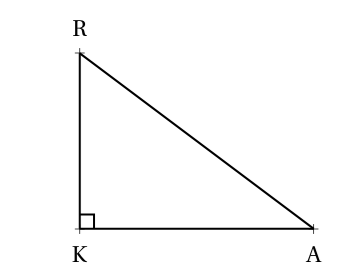
\includegraphics[width=\textwidth]{../../assets/images/4e/seq_02_pythagore/triangle_RKA_rectangle_en_K}
	\end{minipage}
	
	\textbf{Astuce calculatrice :} Utiliser la touche $\sqrt{\phantom{x}}$ ou $x^{1/2}$
\end{examplebox}

\subsection{Calculer la longueur d'un côté de l'angle droit}

\begin{methodebox}[Calculer la longueur d'un côté de l'angle droit]
	Quand on cherche un côté de l'angle droit :
	\begin{enumerate}
		\item Écrire : hypoténuse$^2$ = côté$_1^2$ + côté$_2^2$
		\item Isoler le côté inconnu : côté$_2^2$ = hypoténuse$^2$ - côté$_1^2$
		\item Calculer et prendre la racine carrée
	\end{enumerate}
\end{methodebox}

\begin{examplebox}[Exemple]
	Un triangle $DEF$ est rectangle en $D$. $DE = 5$ cm et $EF = 13$ cm. Calculer $DF$.
	
	\textbf{Solution :}
	\begin{itemize}
		\item Le triangle est rectangle en $D$, donc $EF$ est l'hypoténuse
		\item D'après le théorème de Pythagore : $EF^2 = DE^2 + DF^2$
		\item $13^2 = 5^2 + DF^2$
		\item $169 = 25 + DF^2$
		\item $DF^2 = 169 - 25 = 144$
		\item $DF = \sqrt{144} = 12$ cm
	\end{itemize}
\end{examplebox}

\subsection{Erreurs fréquentes à éviter}

\begin{remarkbox}[Attention aux pièges !]
	\begin{center}
		\begin{tabular}{|l|l|}
			\hline
			\textbf{Erreur courante} & \textbf{Correction} \\
			\hline
			Confondre $2a$ et $a^2$ & $2 \times 5 = 10$ mais $5^2 = 25$ \\
			\hline
			Oublier la racine carrée & Si $x^2 = 36$, alors $x = 6$ (pas 36 !) \\
			\hline
			Se tromper d'hypoténuse & C'est le côté OPPOSÉ à l'angle droit \\
			\hline
			Additionner au lieu de soustraire & Pour un côté : $c^2 = a^2 - b^2$ (pas +) \\
			\hline
		\end{tabular}
	\end{center}
\end{remarkbox}

\section{La réciproque du théorème de Pythagore}

\subsection{Énoncé de la réciproque}

\begin{theoremebox}[Contraposée du théorème de Pythagore]
	\textbf{Si} dans un triangle l'égalité de Pythagore n'est pas vérifiée \textbf{alors} ce triangle n'est pas rectangle.
\end{theoremebox}

\begin{theoremebox}[Réciproque du théorème de Pythagore]
	Si, dans un triangle, le carré de la longueur du plus grand côté est égal à la somme des carrés des longueurs des deux autres côtés, alors ce triangle est rectangle.
	
	\textbf{Autrement dit :} Si $BC^2 = AB^2 + AC^2$ alors le triangle $ABC$ est rectangle en $A$.
\end{theoremebox}

\subsection{Utilisation de la réciproque}

\begin{methodebox}[Démontrer qu'un triangle est rectangle]
	Pour démontrer qu'un triangle est rectangle :
	\begin{enumerate}
		\item Identifier le plus grand côté du triangle
		\item Calculer le carré de sa longueur
		\item Calculer la somme des carrés des deux autres côtés
		\item Comparer les résultats :
		\begin{itemize}
			\item Si égalité : le triangle est rectangle
			\item Si inégalité : le triangle n'est pas rectangle
		\end{itemize}
	\end{enumerate}
\end{methodebox}

\begin{examplebox}[Exemple 1]
	Un triangle a pour côtés 9 cm, 12 cm et 15 cm. Est-il rectangle ?
	
	\textbf{Solution :}
	\begin{itemize}
		\item Le plus grand côté mesure 15 cm
		\item $15^2 = 225$
		\item $9^2 + 12^2 = 81 + 144 = 225$
		\item Puisque $225 = 225$, le triangle est rectangle
		\item L'angle droit est opposé au côté de 15 cm
	\end{itemize}
\end{examplebox}

\begin{examplebox}[Exemple 2]
	Un triangle a pour côtés 7 cm, 8 cm et 10 cm. Est-il rectangle ?
	
	\textbf{Solution :}
	\begin{itemize}
		\item Le plus grand côté mesure 10 cm
		\item $10^2 = 100$
		\item $7^2 + 8^2 = 49 + 64 = 113$
		\item Puisque $100 \neq 113$, le triangle n'est pas rectangle
	\end{itemize}
\end{examplebox}

\section{Applications et résolution de problèmes}

\subsection{Problèmes de la vie courante}

\begin{exercisebox}[L'échelle (sécurité)]
	Une échelle de 4 m est appuyée contre un mur. Son pied est à 1,5 m du mur. À quelle hauteur le sommet de l'échelle touche-t-il le mur ?
	
	\textbf{Résolution :}
	\begin{itemize}
		\item Triangle rectangle : mur-sol-échelle
		\item Hypoténuse : échelle = 4 m
		\item Un côté de l'angle droit : distance au mur = 1,5 m
		\item Autre côté (hauteur) : $h$ = ?
	\end{itemize}
	
	D'après le théorème de Pythagore :
	\begin{align*}
		h^2 + 1,5^2 &= 4^2\\
		h^2 + 2,25 &= 16\\
		h^2 &= 13,75\\
		h &= \sqrt{13,75} \approx 3,71 \text{ m}
	\end{align*}
\end{exercisebox}

\begin{exercisebox}[Vérification d'équerrage (construction)]
	Un maçon vérifie qu'un angle est droit en mesurant les côtés d'un triangle formé par deux murs et une diagonale. Il mesure : 3 m, 4 m et 5 m. L'angle est-il droit ?
	
	\textbf{Solution :}
	\begin{itemize}
		\item Plus grand côté : 5 m donc $5^2 = 25$
		\item Somme des carrés des autres côtés : $3^2 + 4^2 = 9 + 16 = 25$
		\item Égalité vérifiée $(25 = 25)$ $\Rightarrow$ l'angle est droit
	\end{itemize}
\end{exercisebox}

\subsection{Triplets pythagoriciens célèbres}

\begin{definitionbox}[Triplets pythagoriciens]
	Un triplet pythagoricien est un ensemble de trois nombres entiers $(a, b, c)$ tels que $a^2 + b^2 = c^2$.
\end{definitionbox}

\begin{center}
	\begin{tabular}{|c|l|}
		\hline
		\textbf{Triplet} & \textbf{Utilisation historique} \\
		\hline
		$(3, 4, 5)$ & Construction, menuiserie \\
		\hline
		$(5, 12, 13)$ & Architecture égyptienne \\
		\hline
		$(8, 15, 17)$ & Navigation maritime \\
		\hline
		$(7, 24, 25)$ & Arpentage romain \\
		\hline
	\end{tabular}
\end{center}

\section{Exercices différenciés}

\subsection{Niveau 1 - Fondamental}

\begin{exercisebox}
	\textbf{Exercice 1 :} Application directe
	\begin{enumerate}[label=\alph*)]
		\item Triangle rectangle avec côtés de l'angle droit : 6 cm et 8 cm. Calculer l'hypoténuse.
		\item Triangle rectangle avec hypoténuse 5 cm et un côté 3 cm. Calculer l'autre côté.
	\end{enumerate}
	
	\textbf{Exercice 2 :} Vérification
	Est-ce que le triangle de côtés 3 cm, 4 cm et 5 cm est rectangle ?
\end{exercisebox}

\subsection{Niveau 2 - Intermédiaire}

\begin{exercisebox}
	\textbf{Exercice 3 :} Terrain rectangulaire\\
	Un terrain rectangulaire mesure 40 m sur 30 m. Calculer la longueur de sa diagonale.
	
	\textbf{Exercice 4 :} Navigation\\
	Un bateau part d'un port et navigue 12 km vers l'est puis 5 km vers le nord. À quelle distance se trouve-t-il du port ?
\end{exercisebox}

\subsection{Niveau 3 - Expert}

\begin{exercisebox}
	\textbf{Exercice 5 :} Double application\\
	Dans un rectangle $ABCD$, $AB = 12$ cm et $AC = 20$ cm. Calculer $BC$ puis $BD$.
	
	\textbf{Exercice 6 :} Problème ouvert\\
	Un câble de 50 m relie le sommet de deux poteaux verticaux. Le premier poteau mesure 12 m, le second 7 m, et ils sont distants de 40 m. Le câble touche-t-il le sol entre les deux poteaux ?
\end{exercisebox}

\begin{exercisebox}[Défi bonus]
	Trouver tous les triangles rectangles dont les trois côtés sont des nombres entiers inférieurs à 20.
\end{exercisebox}

\section{Auto-évaluation}

\subsection*{QCM - Testez vos connaissances}

\begin{enumerate}
	\item Dans un triangle rectangle, l'hypoténuse est :
	\begin{itemize}
		\item[$\square$] Un côté de l'angle droit
		\item[$\square$] Le plus petit côté
		\item[$\square$] Le côté opposé à l'angle droit
	\end{itemize}
	
	\item Si un triangle a pour côtés 6, 8 et 10 :
	\begin{itemize}
		\item[$\square$] Il est rectangle
		\item[$\square$] Il n'est pas rectangle
		\item[$\square$] On ne peut pas savoir
	\end{itemize}
	
	\item $\sqrt{49}$ est égal à :
	\begin{itemize}
		\item[$\square$] 24,5
		\item[$\square$] 7
		\item[$\square$] 14
	\end{itemize}
\end{enumerate}

\subsection*{Carte mentale à compléter}

\begin{center}
	\fbox{\parbox{14cm}{
			\textbf{THÉORÈME DE PYTHAGORE}
			
			\vspace{0.5cm}
			\textbf{1. Dans un triangle rectangle}
			\begin{itemize}
				\item Hypoténuse² = \trous{5cm}
				\item Permet de calculer \trous{5cm}
			\end{itemize}
			
			\vspace{0.3cm}
			\textbf{2. Réciproque}
			\begin{itemize}
				\item Si \trous{5cm} alors \trous{5cm}
				\item Permet de vérifier \trous{5cm}
			\end{itemize}
			
			\vspace{0.3cm}
			\textbf{3. Applications}
			\begin{itemize}
				\item Construction et architecture
				\item Navigation et cartographie
				\item \trous{5cm}
			\end{itemize}
	}}
\end{center}

\section{Pour aller plus loin}

\subsection{Lien avec les identités remarquables}
Le théorème de Pythagore utilise $a^2 + b^2 = c^2$, qui ressemble aux identités remarquables étudiées en calcul littéral ! 

Par exemple : $(a + b)^2 = a^2 + 2ab + b^2$ nous a servi dans la démonstration.

\subsection{Culture mathématique}
\begin{itemize}
	\item Il existe plus de 400 démonstrations différentes du théorème de Pythagore !
	\item Einstein en a proposé une à l'âge de 12 ans.
	\item Le théorème se généralise en dimension 3 : dans un parallélépipède rectangle, la diagonale $d$ vérifie $d^2 = a^2 + b^2 + c^2$.
\end{itemize}

\subsection{Projet interdisciplinaire}
\begin{itemize}
	\item \textbf{Technologie :} Programmer un vérificateur de triangle rectangle avec Scratch
	\item \textbf{Arts plastiques :} Créer une œuvre basée sur les triplets pythagoriciens
	\item \textbf{Histoire :} Rechercher l'utilisation du théorème dans les monuments de votre région
	\item \textbf{EPS :} Calculer les distances réelles sur un terrain de sport
\end{itemize}

\section*{Ressources supplémentaires}
\begin{itemize}
	\item \textbf{Vidéos :} Animations GeoGebra interactives disponibles sur le site du collège
	\item \textbf{Exercices en ligne :} Auto-correction disponible sur Pronote
	\item \textbf{Aide :} Fiches méthodes téléchargeables
	\item \textbf{Pour les curieux :} <<Le théorème de Pythagore en dimension $n$>>
\end{itemize}

\section{Corrigés détaillés des exercices}

\subsection{Niveau 1 - Fondamental}

\begin{exercisebox}[Corrigé Exercice 1]
	\textbf{a) Triangle rectangle avec côtés 6 cm et 8 cm}
	
	Solution :
	\begin{itemize}
		\item Triangle rectangle, hypoténuse = $h$
		\item D'après Pythagore : $h^2 = 6^2 + 8^2$
		\item $h^2 = 36 + 64 = 100$
		\item $h = \sqrt{100} = 10$ cm
	\end{itemize}
	
	\textbf{b) Triangle rectangle, hypoténuse 5 cm, un côté 3 cm}
	
	Solution :
	\begin{itemize}
		\item Soit $x$ le côté inconnu
		\item D'après Pythagore : $5^2 = 3^2 + x^2$
		\item $25 = 9 + x^2$
		\item $x^2 = 16$
		\item $x = \sqrt{16} = 4$ cm
	\end{itemize}
	
	\textbf{Exercice 2 : Triangle 3-4-5}
	\begin{itemize}
		\item Plus grand côté : 5 cm $\Rightarrow 5^2 = 25$
		\item Autres côtés : $3^2 + 4^2 = 9 + 16 = 25$
		\item $25 = 25$ $\Rightarrow$ Le triangle est rectangle
	\end{itemize}
\end{exercisebox}

\subsection{Niveau 2 - Intermédiaire}

\begin{exercisebox}[Corrigé Exercice 3]
	\textbf{Terrain rectangulaire 40 m × 30 m}
	
	Solution :
	\begin{itemize}
		\item Le terrain rectangulaire forme un angle droit
		\item La diagonale $d$ est l'hypoténuse du triangle rectangle
		\item D'après le théorème de Pythagore : $d^2 = 40^2 + 30^2$
		\item $d^2 = 1600 + 900 = 2500$
		\item $d = \sqrt{2500} = 50$ m
	\end{itemize}
	
	\textbf{Exercice 4 : Navigation}
	\begin{itemize}
		\item Déplacement Est : 12 km
		\item Déplacement Nord : 5 km (perpendiculaire)
		\item Distance au port : $d^2 = 12^2 + 5^2 = 144 + 25 = 169$
		\item $d = \sqrt{169} = 13$ km
	\end{itemize}
\end{exercisebox}

\subsection{Niveau 3 - Expert}

\begin{exercisebox}[Corrigé Exercice 5]
	\textbf{Rectangle ABCD avec AB = 12 cm et AC = 20 cm}
	
	\textbf{Étape 1 : Calculer BC}
	\begin{itemize}
		\item Triangle ABC rectangle en B
		\item $AC^2 = AB^2 + BC^2$
		\item $20^2 = 12^2 + BC^2$
		\item $400 = 144 + BC^2$
		\item $BC^2 = 256$
		\item $BC = \sqrt{256} = 16$ cm
	\end{itemize}
	
	\textbf{Étape 2 : Calculer BD}
	\begin{itemize}
		\item Dans un rectangle, les diagonales sont égales
		\item Donc $BD = AC = 20$ cm
		\item Vérification : $BD^2 = BC^2 + CD^2 = 16^2 + 12^2 = 256 + 144 = 400$
		\item $BD = \sqrt{400} = 20$ cm ✓
	\end{itemize}
	
	\textbf{Exercice 6 : Problème du câble}
	
	Analyse :
	\begin{itemize}
		\item Distance horizontale : 40 m
		\item Différence de hauteur : $12 - 7 = 5$ m
		\item Distance minimale nécessaire : $\sqrt{40^2 + 5^2} = \sqrt{1600 + 25} = \sqrt{1625} \approx 40,31$ m
		\item Longueur du câble : 50 m
		\item $50 > 40,31$ $\Rightarrow$ Le câble a du mou et touchera le sol
	\end{itemize}
\end{exercisebox}

\begin{exercisebox}[Corrigé Défi bonus]
	\textbf{Triplets pythagoriciens avec côtés < 20}
	
	\begin{center}
		\begin{tabular}{|c|c|c|c|}
			\hline
			\textbf{a} & \textbf{b} & \textbf{c} & \textbf{Vérification} \\
			\hline
			3 & 4 & 5 & $9 + 16 = 25$ ✓ \\
			5 & 12 & 13 & $25 + 144 = 169$ ✓ \\
			6 & 8 & 10 & $36 + 64 = 100$ ✓ \\
			8 & 15 & 17 & $64 + 225 = 289$ ✓ \\
			9 & 12 & 15 & $81 + 144 = 225$ ✓ \\
			12 & 16 & 20 & Non (20 n'est pas < 20) \\
			\hline
		\end{tabular}
	\end{center}
	
	\textbf{Réponse :} Il existe 5 triangles rectangles à côtés entiers < 20.
\end{exercisebox}

\section{Fiches méthodes}

\begin{methodebox}[Fiche méthode 1 : Organiser ses calculs]
	\textbf{Pour l'hypoténuse :}
	\begin{verbatim}
		Données : Triangle ... rectangle en ...
		Côté 1 = ... cm
		Côté 2 = ... cm
		
		Calcul : hyp² = côté1² + côté2²
		hyp² = ...² + ...²
		hyp² = ... + ...
		hyp² = ...
		hyp = √... = ... cm
	\end{verbatim}
	
	\textbf{Pour un côté de l'angle droit :}
	\begin{verbatim}
		Données : Triangle ... rectangle en ...
		Hypoténuse = ... cm
		Côté connu = ... cm
		
		Calcul : hyp² = côté1² + côté2²
		...² = ...² + côté2²
		... = ... + côté2²
		côté2² = ... - ...
		côté2² = ...
		côté2 = √... = ... cm
	\end{verbatim}
\end{methodebox}

\begin{methodebox}[Fiche méthode 2 : Utiliser la calculatrice]
	\textbf{Pour calculer un carré :}
	\begin{itemize}
		\item Taper le nombre
		\item Appuyer sur $x^2$ ou utiliser $\times$ puis =
		\item Exemple : $7^2$ → 7 [x²] → 49
	\end{itemize}
	
	\textbf{Pour calculer une racine carrée :}
	\begin{itemize}
		\item Appuyer sur $\sqrt{\phantom{x}}$
		\item Taper le nombre
		\item Appuyer sur =
		\item Exemple : $\sqrt{169}$ → [√] 169 [=] → 13
	\end{itemize}
	
	\textbf{Pour un calcul complet :}
	\begin{itemize}
		\item $\sqrt{12^2 + 5^2}$ → [√] ( 12 [x²] + 5 [x²] ) [=] → 13
	\end{itemize}
\end{methodebox}

\section{Activités complémentaires}

\subsection{Activité 1 : Construction à la règle et au compas}

\begin{exercisebox}[Construction d'un angle droit]
	\textbf{Matériel :} Règle graduée, compas
	
	\textbf{Méthode des Égyptiens (corde à 12 nœuds) :}
	\begin{enumerate}
		\item Tracer un segment [AB] de 4 cm
		\item Depuis A, tracer un arc de cercle de rayon 5 cm
		\item Depuis B, tracer un arc de cercle de rayon 3 cm
		\item Les deux arcs se coupent en C
		\item Le triangle ABC est rectangle en B
	\end{enumerate}
	
	\textbf{Vérification :} Mesurer et vérifier que $5^2 = 3^2 + 4^2$
\end{exercisebox}

\subsection{Activité 2 : Pythagore dans l'espace}

\begin{exercisebox}[Extension en 3D]
	Dans un parallélépipède rectangle de dimensions $a$, $b$ et $c$, la diagonale principale $d$ vérifie :
	$d^2 = a^2 + b^2 + c^2$
	
	\textbf{Application :} Une boîte mesure 3 cm × 4 cm × 12 cm. 
	\begin{itemize}
		\item Diagonale de la base : $\sqrt{3^2 + 4^2} = 5$ cm
		\item Diagonale principale : $\sqrt{3^2 + 4^2 + 12^2} = \sqrt{9 + 16 + 144} = \sqrt{169} = 13$ cm
	\end{itemize}
\end{exercisebox}

\subsection{Activité 3 : Programmation Scratch}

\begin{exercisebox}[Créer un vérificateur de triangle rectangle]
	\textbf{Algorithme :}
	\begin{verbatim}
		DÉBUT
		Demander "Côté 1 ?" → a
		Demander "Côté 2 ?" → b  
		Demander "Côté 3 ?" → c
		
		Trouver le maximum → max
		Calculer la somme des carrés des deux autres → somme
		
		SI max² = somme ALORS
		Dire "Le triangle est rectangle"
		SINON
		Dire "Le triangle n'est pas rectangle"
		FIN SI
		FIN
	\end{verbatim}
\end{exercisebox}

\section{Évaluation formative}

\subsection{Grille d'auto-évaluation}

\begin{center}
	\begin{tabular}{|l|c|c|c|c|}
		\hline
		\textbf{Compétence} & \textbf{Non acquis} & \textbf{En cours} & \textbf{Acquis} & \textbf{Expert} \\
		\hline
		Je sais identifier l'hypoténuse & $\square$ & $\square$ & $\square$ & $\square$ \\
		\hline
		Je sais écrire l'égalité de Pythagore & $\square$ & $\square$ & $\square$ & $\square$ \\
		\hline
		Je sais calculer un carré & $\square$ & $\square$ & $\square$ & $\square$ \\
		\hline
		Je sais calculer une racine carrée & $\square$ & $\square$ & $\square$ & $\square$ \\
		\hline
		Je sais calculer l'hypoténuse & $\square$ & $\square$ & $\square$ & $\square$ \\
		\hline
		Je sais calculer un côté de l'angle droit & $\square$ & $\square$ & $\square$ & $\square$ \\
		\hline
		Je sais vérifier qu'un triangle est rectangle & $\square$ & $\square$ & $\square$ & $\square$ \\
		\hline
		Je sais résoudre un problème concret & $\square$ & $\square$ & $\square$ & $\square$ \\
		\hline
	\end{tabular}
\end{center}

\subsection{Mini-test de positionnement}

\begin{exercisebox}[Test rapide - 10 minutes]
	\textbf{Question 1 (2 points) :} Un triangle ABC est rectangle en A. AB = 3 cm et AC = 4 cm. Calculer BC.
	
	\vspace{3cm}
	
	\textbf{Question 2 (2 points) :} Un triangle a pour côtés 7 cm, 24 cm et 25 cm. Est-il rectangle ?
	
	\vspace{3cm}
	
	\textbf{Question 3 (3 points) :} Une échelle de 5 m est posée contre un mur. Son pied est à 3 m du mur. À quelle hauteur arrive-t-elle ?
	
	\vspace{3cm}
	
	\textbf{Question 4 (3 points) :} Dans un carré de côté 10 cm, calculer la longueur de la diagonale.
	
	\vspace{3cm}
	
	\textbf{Barème :}
	\begin{itemize}
		\item 8-10 points : Excellent !
		\item 6-7 points : Bien, quelques révisions nécessaires
		\item 4-5 points : Des efforts à poursuivre
		\item < 4 points : Revoir le cours et demander de l'aide
	\end{itemize}
\end{exercisebox} % Théorème de Pythagore
% Chapitre 3 : Calcul littéral (I) - Expressions et développement
% Conforme à la réforme du collège 2025
% Note: Ce document nécessite les packages tikz, amsmath, amssymb et les environnements personnalisés définis dans le préambule

\chapter{Calcul littéral (I) : Expressions et simple distributivité}

\section{Introduction}

Le calcul littéral est le langage universel des mathématiques. Il permet d'exprimer des relations générales, de modéliser des situations et de résoudre des problèmes complexes.

\subsection*{Un peu d'histoire}
\begin{itemize}
	\item \textbf{Al-Khwarizmi (IXe siècle)} : Père de l'algèbre, introduit la résolution systématique d'équations.
	\item \textbf{François Viète (XVIe siècle)} : Premier à utiliser des lettres pour représenter des nombres inconnus et connus.
	\item \textbf{René Descartes (XVIIe siècle)} : Normalise l'usage de $x$, $y$, $z$ pour les inconnues et $a$, $b$, $c$ pour les paramètres.
\end{itemize}

\textbf{Problématique du chapitre :} Comment traduire une situation par une expression mathématique ? Comment simplifier et transformer des expressions pour faciliter les calculs ?

\section{Activité — Du langage courant au langage mathématique}

\begin{objectifsbox}
	\begin{itemize}
		\item[\textbullet] Traduire une situation concrète en expression littérale
		\item[\textbullet] Comprendre l'utilité des lettres en mathématiques
		\item[\textbullet] Découvrir les règles de simplification
	\end{itemize}
\end{objectifsbox}

\subsection*{Situation 1 : Le périmètre d'un terrain}

\begin{activitybox}[Les dimensions variables]
	Un terrain rectangulaire a une longueur de 20 mètres de plus que sa largeur.
	
	\begin{enumerate}
		\item Si la largeur mesure 30 m, quelle est la longueur ? \trous{3cm}
		\item Si la largeur mesure 45 m, quelle est la longueur ? \trous{3cm}
		\item Si on note $\ell$ la largeur, comment exprimer la longueur ? \trous{5cm}
		\item Exprimer le périmètre du terrain en fonction de $\ell$ : \trous{8cm}
		\item Simplifier cette expression : \trous{8cm}
	\end{enumerate}
\end{activitybox}

\subsection*{Situation 2 : Tarifs et réductions}

\begin{activitybox}[Modélisation d'une situation commerciale]
	Un magasin propose une réduction de 20\% sur tous les articles.
	
	\begin{enumerate}
		\item Si un article coûte 50€, quel est son prix après réduction ? \trous{3cm}
		\item Si un article coûte $p$ euros, exprimer :
		\begin{itemize}
			\item Le montant de la réduction : \trous{5cm}
			\item Le prix après réduction : \trous{5cm}
		\end{itemize}
		\item Simplifier l'expression du prix après réduction : \trous{5cm}
	\end{enumerate}
\end{activitybox}

\section{Vocabulaire et notations}

\begin{definitionbox}[Expression littérale]
	Une \textbf{expression littérale} est une expression mathématique comportant une ou plusieurs lettres qui représentent des nombres.
	
	\textbf{Exemples :} $3x + 5$, $2a - b$, $x^2 + 2x - 3$
	
	Les lettres utilisées sont appelées \textbf{variables} ou \textbf{inconnues}.
\end{definitionbox}

\begin{vocabulairebox}[Terminologie du calcul littéral]
	\begin{itemize}
		\item \textbf{Terme} : Partie d'une expression séparée par + ou -
		\begin{itemize}
			\item[\textbullet] Dans $3x + 5y - 2$, les termes sont : \solution{$3x$}, \solution{$5y$} et \solution{$-2$}
		\end{itemize}
		\item \textbf{Coefficient} : Nombre qui multiplie une variable
		\begin{itemize}
			\item[\textbullet] Dans $7x$, le coefficient est \solution{7}
			\item[\textbullet] Dans $-3y$, le coefficient est \solution{-3}
			\item[\textbullet] Dans $x$, le coefficient est \solution{1} (sous-entendu)
		\end{itemize}
		\item \textbf{Partie littérale} : La ou les lettres d'un terme
		\begin{itemize}
			\item[\textbullet] Dans $5xy$, la partie littérale est \solution{$xy$}
		\end{itemize}
		\item \textbf{Terme constant} : Terme sans variable
		\begin{itemize}
			\item[\textbullet] Dans $2x + 8$, le terme constant est \solution{8}
		\end{itemize}
	\end{itemize}
\end{vocabulairebox}

\begin{remarkbox}[Conventions d'écriture]
	\begin{itemize}
		\item[\textbullet] Le signe $\times$ est souvent omis : $3 \times x = 3x$
		\item[\textbullet] $1 \times x = x$ (on n'écrit pas le coefficient 1)
		\item[\textbullet] $-1 \times x = -x$ (on n'écrit pas le coefficient -1)
		\item[\textbullet] Entre deux lettres : $a \times b = ab$
		\item[\textbullet] Ordre alphabétique préféré : $xy$ plutôt que $yx$
	\end{itemize}
\end{remarkbox}

\section{Calculer la valeur d'une expression}

\begin{definitionbox}[Substitution]
	\textbf{Substituer}, c'est remplacer une lettre par une valeur numérique donnée.
	
	Pour calculer la valeur d'une expression littérale :
	\begin{enumerate}
		\item Remplacer chaque lettre par sa valeur
		\item Respecter les priorités opératoires
		\item Effectuer les calculs
	\end{enumerate}
\end{definitionbox}

\begin{methodebox}[Calculer une valeur numérique]
	\textbf{Étapes à suivre :}
	\begin{enumerate}
		\item Réécrire l'expression en remplaçant les lettres par leurs valeurs (entre parenthèses si nécessaire)
		\item Appliquer les priorités : Parenthèses → Puissances → Multiplications/Divisions → Additions/Soustractions
		\item Calculer progressivement
	\end{enumerate}
\end{methodebox}

\begin{examplebox}[Substitution simple]
	Calculer $A = 3x - 5$ pour $x = 4$
	
	\textbf{Solution :}
	\begin{align*}
		A &= 3x - 5\\
		A &= ..........\\
		A &= ...........\\
		A &= ...........
	\end{align*}
\end{examplebox}

\begin{examplebox}[Substitution avec plusieurs variables]
	Calculer $B = 2a + 3b - ab$ pour $a = 5$ et $b = -2$
	
	\textbf{Solution :}
	\begin{align*}
		B &= 2a + 3b - ab\\
		B &= .......................................\\
		B &= ............................\\
		B &= ............................\\
		B &= ............................
	\end{align*}
\end{examplebox}

\begin{attentionbox}[Piège des nombres négatifs]
	Attention lors de la substitution de nombres négatifs !
	
	Si $x = -3$ :
	\begin{itemize}
		\item $x^2 = (-3)^2 = 9$ (et non pas $-9$)
		\item $2x = 2 \times (-3) = -6$
		\item $-x = -(-3) = 3$
	\end{itemize}
	
	\textbf{Conseil :} Mettre les nombres négatifs entre parenthèses lors de la substitution.
\end{attentionbox}

\section{Simplifier et réduire une expression}

\subsection{Simplifier une écriture}

\begin{definitionbox}[Simplification]
	\textbf{Simplifier} une expression, c'est l'écrire de la manière la plus concise possible en respectant les conventions mathématiques.
\end{definitionbox}

\begin{examplebox}[Simplifications courantes]
	\begin{center}
		\begin{tabular}{|l|l|l|}
			\hline
			\textbf{Écriture non simplifiée} & \textbf{Écriture simplifiée} & \textbf{Règle appliquée} \\
			\hline
			$1 \times x$ & $x$ & Coefficient 1 omis \\
			\hline
			$x \times 3$ & $3x$ & Coefficient devant \\
			\hline
			$x \times y$ & $xy$ & Signe $\times$ omis \\
			\hline
			$x + (-5)$ & $x - 5$ & Simplification des signes \\
			\hline
			$0 \times x$ & $0$ & Multiplication par 0 \\
			\hline
			$x + 0$ & $x$ & Addition de 0 \\
			\hline
		\end{tabular}
	\end{center}
\end{examplebox}

\subsection{Réduire une expression}

\begin{definitionbox}[Réduction]
	\textbf{Réduire} une expression, c'est regrouper les termes qui ont la même partie littérale (termes semblables).
\end{definitionbox}

\begin{proprietebox}[Termes semblables]
	Deux termes sont semblables s'ils ont exactement la même partie littérale.
	
	\textbf{Exemples :}
	\begin{itemize}
		\item $3x$ et $5x$ sont semblables (partie littérale : $x$)
		\item $2xy$ et $-7xy$ \solution[5cm]{sont semblables (partie littérale : $xy$)}
		\item $4x$ et $4y$ \solution[6cm]{ne sont PAS semblables}
		\item $3x^2$ et $3x$ \solution[6cm]{ne sont PAS semblables}
	\end{itemize}
\end{proprietebox}

\begin{methodebox}[Réduire une expression]
	\textbf{Méthode systématique :}
	\begin{enumerate}
		\item Identifier les termes semblables (même partie littérale)
		\item Les regrouper mentalement ou les souligner de la même couleur
		\item Additionner ou soustraire leurs coefficients
		\item Écrire l'expression réduite
	\end{enumerate}
\end{methodebox}

\begin{examplebox}[Réduction guidée]
	Réduire $E = 5x + 3y - 2x + y - 4$
	
	\textbf{Solution détaillée :}
	\begin{itemize}
		\item Termes en $x$ : $5x$ et $-2x$ → $(5 - 2)x = 3x$
		\item Termes en $y$ : $3y$ et $y$ → $(3 + 1)y = 4y$
		\item Terme constant : $-4$
		\item \textbf{Résultat :} $E = 3x + 4y - 4$
	\end{itemize}
\end{examplebox}

\begin{examplebox}[Réduction complexe]
	Réduire $F = 2a^2 + 3a - 5 + a^2 - 7a + 2$
	
	\textbf{Solution :}
	\begin{itemize}
		\item Termes en $a^2$ : \solution{$2a^2$} et \solution{$a^2$} → \solution{$(2 + 1)a^2 = 3a^2$}
		\item Termes en $a$ : \solution{$3a$} et \solution{$-7a$} → \solution{$(3 - 7)a = -4a$}
		\item Termes constants : \solution{$-5$} et \solution{$2$} → \solution{$-5 + 2 = -3$}
		\item \textbf{Résultat :} $F = \solution{3a^2 - 4a - 3}$
	\end{itemize}
\end{examplebox}

\section{Développer avec la distributivité simple}

\begin{definitionbox}[Développer une expression]
	\textbf{Développer} une expression, c'est transformer un produit en une somme algébrique.

	On passe d'une forme factorisée (produit) à une forme développée (somme).

	\textbf{Exemple :} $2(x + 3)$ (produit) $\longrightarrow$ $2x + 6$ (somme)
\end{definitionbox}

\begin{examplebox}[Pourquoi développer ?]
	Calculer $3(x + 5)$ pour $x = 2$ :

	\textbf{Méthode 1 (sans développer) :}
	$$\solution{3(2 + 5)} = \solution{3 \times 7 = 21}$$

	\textbf{Méthode 2 (en développant) :}
	$$3(x + 5) = \solution{3x + 15}$$
	donc pour $x = 2$ : $3 \times 2 + 15 = 6 + 15 = 21$
	
	Développer permet de transformer l'expression et facilite certains calculs ultérieurs.
\end{examplebox}

\subsection{La propriété de distributivité}

\begin{proprietebox}[Distributivité de la multiplication]
	Pour tous nombres $k$, $a$ et $b$ :
	\begin{itemize}
		\item $k(a + b) = ka + kb$ \quad (distributivité sur l'addition)
		\item $k(a - b) = ka - kb$ \quad (distributivité sur la soustraction)
	\end{itemize}

	\textbf{Visualisation géométrique :}
	\begin{center}
		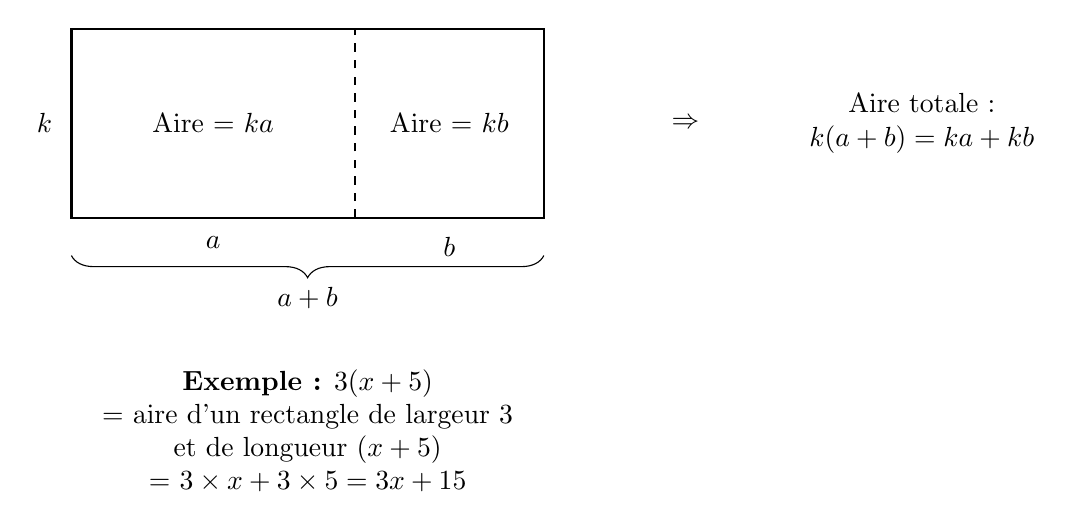
\begin{tikzpicture}[scale=1.2]
			% Rectangle principal
			\draw[thick] (0,0) rectangle (5,2);

			% Séparation verticale
			\draw[dashed, thick] (3,0) -- (3,2);

			% Labels des dimensions
			\node[below] at (1.5,-0.1) {$a$};
			\node[below] at (4,-0.1) {$b$};
			\node[left] at (-0.1,1) {$k$};

			% Accolades pour montrer a+b
			\draw[decorate, decoration={brace, amplitude=8pt, mirror}]
				(0,-0.4) -- (5,-0.4) node[midway, below, yshift=-8pt] {$a + b$};

			% Labels des aires
			\node at (1.5,1) {Aire = $ka$};
			\node at (4,1) {Aire = $kb$};

			% Flèche et égalité
			\node at (6.5,1) {$\Rightarrow$};
			\node[align=center] at (9,1) {Aire totale :\\ \solution{$k(a+b) = ka + kb$}};

			% Exemple numérique en dessous
			\node[below, align=center] at (2.5,-1.5) {
				\textbf{Exemple :} $3(x + 5)$\\
				= aire d'un rectangle de largeur 3\\
				et de longueur $(x + 5)$\\
				= $3 \times x + 3 \times 5 = 3x + 15$
			};
		\end{tikzpicture}
	\end{center}
\end{proprietebox}

\begin{remarkbox}[Sens de lecture]
	\begin{itemize}
		\item \textbf{Développer :} passer de $k(a + b)$ à $ka + kb$
		\item \textbf{Factoriser :} passer de $ka + kb$ à $k(a + b)$ (vu plus tard)
	\end{itemize}
\end{remarkbox}

\begin{methodebox}[Développer une expression]
	Pour développer $k(a + b)$ :
	\begin{enumerate}
		\item Multiplier $k$ par chaque terme dans la parenthèse
		\item Respecter la règle des signes
		\item Simplifier si possible
		\item Réduire l'expression obtenue
	\end{enumerate}
\end{methodebox}

\begin{examplebox}[Développement simple]
	Développer $A = 3(x + 5)$
	
	\textbf{Solution :}
	\begin{align*}
		A &= 3(x + 5)\\
		A &= \solution{3 \times x + 3 \times 5}\\
		A &= \solution{3x + 15}
	\end{align*}
\end{examplebox}

\begin{examplebox}[Développement avec soustraction]
	Développer $B = 4(2x - 3)$
	
	\textbf{Solution :}
	\begin{align*}
		B &= 4(2x - 3)\\
		B &= \solution{4 \times 2x - 4 \times 3}\\
		B &= \solution{8x - 12}
	\end{align*}
\end{examplebox}

\begin{examplebox}[Développement avec coefficient négatif]
	Développer $C = -2(3x + 4)$
	
	\textbf{Solution :}
	\begin{align*}
		C &= -2(3x + 4)\\
		C &= \solution{-2 \times 3x + (-2) \times 4}\\
		C &= \solution{-6x - 8}
	\end{align*}
\end{examplebox}

\begin{attentionbox}[Erreurs fréquentes]
	\begin{center}
		\begin{tabular}{|l|l|l|}
			\hline
			\textbf{Erreur} & \textbf{Faux} & \textbf{Correct} \\
			\hline
			Oubli d'un terme & $3(x + 2) = 3x$ & $3(x + 2) =$ \solution{$3x + 6$} \\
			\hline
			Erreur de signe & $-2(x - 3) = -2x - 6$ & $-2(x - 3) =$ \solution{$-2x + 6$} \\
			\hline
			Distribution partielle & $2(3x + 4y) = 6x + 4y$ & $2(3x + 4y) = \solution{6x + 8y}$ \\
			\hline
		\end{tabular}
	\end{center}
\end{attentionbox}

\subsection{Développement et réduction}

\begin{methodebox}[Développer puis réduire]
	Quand une expression contient plusieurs développements :
	\begin{enumerate}
		\item Développer chaque produit séparément
		\item Supprimer toutes les parenthèses
		\item Identifier les termes semblables
		\item Réduire l'expression
	\end{enumerate}
\end{methodebox}

\begin{examplebox}[Exemple complet]
	Développer et réduire $D = 3(x + 2) + 2(x - 4)$
	
	\textbf{Solution détaillée :}
	\begin{align*}
		D &= 3(x + 2) + 2(x - 4)\\
		&= 3x + 6 + 2x - 8 \quad \text{(développement)}\\
		&= 3x + 2x + 6 - 8 \quad \text{(regroupement)}\\
		&= 5x - 2 \quad \text{(réduction)}
	\end{align*}
\end{examplebox}

\begin{examplebox}[Avec coefficients négatifs]
	Développer et réduire $E = -2(x + 3) + 4(2 - x)$
	
	\textbf{Solution :}
	\begin{align*}
		E &= -2(x + 3) + 4(2 - x)\\
		&= \solution{-2x - 6 + 8 - 4x}\\
		&= \solution{-2x - 4x - 6 + 8}\\
		&= \solution{-6x + 2}
	\end{align*}
\end{examplebox}

\section{Applications et modélisation}

\subsection{Problèmes géométriques}

\begin{applicationbox}[Périmètres et aires]
	\textbf{Situation :} Un rectangle a une longueur égale au double de sa largeur plus 3 cm.
	
	Si on note $x$ la largeur :
	\begin{itemize}
		\item Longueur = \solution{$2x + 3$}
		\item Périmètre = $\solution[4cm]{2(x + 2x + 3)} = \solution[4cm]{2(3x + 3)} = \solution{6x + 6}$
		\item Aire = $\solution{x(2x + 3)} = \solution{2x^2 + 3x}$
	\end{itemize}
	
	\textbf{Application numérique :} Si $x = 5$ cm
	\begin{itemize}
		\item Périmètre = $\solution[3cm]{6 \times 5 + 6} = \solution{36}$ cm
		\item Aire = \solution{$2 \times 25 + 3 \times 5 = 50 + 15 = 65 \ cm^2$}
	\end{itemize}
\end{applicationbox}

\subsection{Problèmes de la vie courante}

\begin{applicationbox}[Tarification]
	Un taxi facture 3€ de prise en charge puis 1,50€ par kilomètre.
	
	\textbf{Expression du prix :} $P = \solution[4cm]{3 + 1,5d}$ où $d$ est la distance en km
	
	\textbf{Questions :}
	\begin{enumerate}
		\item Prix pour 10 km : $P = \solution[4cm]{3 + 1,5 \times 10} = \solution{18}$€
		\item Si le client paie 30€, quelle distance a-t-il parcourue ?
		\begin{align*}
			\solution{30} &= \solution{3 + 1,5d}\\
			\solution{27} &= \solution{1,5d}\\
			d &= \solution{18} \text{ km}
		\end{align*}
	\end{enumerate}
\end{applicationbox}

\section{Exercices différenciés}

\subsection{Niveau 1 - Fondamental}

\begin{exercisebox}
	\textbf{Exercice 1 :} Simplifier les expressions
	\begin{enumerate}[label=\alph*)]
		\item $1 \times x + 3$ = \trous{3cm}
		\item $y \times 5 - 2 \times y$ = \trous{3cm}
		\item $a + 0 + b \times 1$ = \trous{3cm}
	\end{enumerate}
	
	\textbf{Exercice 2 :} Calculer pour $x = 3$
	\begin{enumerate}[label=\alph*)]
		\item $A = 2x + 5$ = \trous{3cm}
		\item $B = x^2 - 4$ = \trous{3cm}
		\item $C = 3(x - 1)$ = \trous{3cm}
	\end{enumerate}
	
	\textbf{Exercice 3 :} Réduire
	\begin{enumerate}[label=\alph*)]
		\item $3x + 2x$ = \trous{3cm}
		\item $5y - 3y + y$ = \trous{3cm}
		\item $4a + 2 - a + 3$ = \trous{3cm}
	\end{enumerate}
\end{exercisebox}

\subsection{Niveau 2 - Intermédiaire}

\begin{exercisebox}
	\textbf{Exercice 4 :} Réduire les expressions
	\begin{enumerate}[label=\alph*)]
		\item $A = 3x + 2y - x + 4y - 5$
		\item $B = 2a^2 + 3a - a^2 + 5a - 7$
		\item $C = 4xy - 2x + 3xy + x$
	\end{enumerate}
	
	\textbf{Exercice 5 :} Développer
	\begin{enumerate}[label=\alph*)]
		\item $D = 3(x + 4)$
		\item $E = -2(3x - 5)$
		\item $F = 4(2a + 3b)$
	\end{enumerate}
	
	\textbf{Exercice 6 :} Développer et réduire
	\begin{enumerate}[label=\alph*)]
		\item $G = 2(x + 3) + 3(x - 1)$
		\item $H = 5(y - 2) - 2(y + 4)$
	\end{enumerate}
\end{exercisebox}

\subsection{Niveau 3 - Expert}

\begin{exercisebox}
	\textbf{Exercice 7 :} Expressions complexes
	
	Développer et réduire :
	\begin{enumerate}[label=\alph*)]
		\item $I = 3(2x - 1) - 2(3x + 4) + 5$
		\item $J = -4(a - 2b) + 3(2a + b) - (a - 3b)$
	\end{enumerate}
	
	\textbf{Exercice 8 :} Problème ouvert
	
	Un carré a pour côté $(x + 3)$ cm.
	\begin{enumerate}
		\item Exprimer son périmètre en fonction de $x$
		\item Exprimer son aire en fonction de $x$ (développer)
		\item Pour quelle valeur de $x$ le périmètre vaut-il 28 cm ?
		\item Calculer alors l'aire du carré
	\end{enumerate}
\end{exercisebox}

\begin{exercisebox}[Défi bonus]
	On considère trois nombres entiers consécutifs. Le plus petit est noté $n$.
	\begin{enumerate}
		\item Exprimer les deux autres en fonction de $n$
		\item Montrer que leur somme peut s'écrire $3n + 3$
		\item En déduire que la somme de trois entiers consécutifs est toujours divisible par 3
	\end{enumerate}
\end{exercisebox}

\section{Programme de construction}

\begin{activitybox}[Créer et interpréter]
	\textbf{Programme A :}
	\begin{enumerate}
		\item Choisir un nombre
		\item Le multiplier par 2
		\item Ajouter 5
		\item Multiplier le résultat par 3
	\end{enumerate}
	
	\textbf{Questions :}
	\begin{enumerate}[label=\alph*)]
		\item Tester avec 4, puis avec -2
		\item Si on note $x$ le nombre choisi, exprimer le résultat final
		\item Développer et simplifier cette expression
		\item Pour quelle valeur de $x$ obtient-on 45 ?
	\end{enumerate}
\end{activitybox}

\section{Auto-évaluation}

\subsection{QCM de vérification}

\begin{quizbox}
	\begin{enumerate}
		\item L'expression $3x + 2x$ est égale à :
		\begin{itemize}
			\item[$\square$] $5x^2$
			\item[$\square$] $5x$
			\item[$\square$] $6x$
		\end{itemize}
		
		\item Le développement de $-3(x - 2)$ est :
		\begin{itemize}
			\item[$\square$] $-3x - 6$
			\item[$\square$] $-3x + 6$
			\item[$\square$] $-3x - 2$
		\end{itemize}
		
		\item Pour $x = -2$, l'expression $x^2 - 3x$ vaut :
		\begin{itemize}
			\item[$\square$] $-2$
			\item[$\square$] $10$
			\item[$\square$] $-10$
		\end{itemize}
		
		\item Les termes $3xy$ et $3yx$ :
		\begin{itemize}
			\item[$\square$] Sont semblables
			\item[$\square$] Ne sont pas semblables
			\item[$\square$] On ne peut pas savoir
		\end{itemize}
	\end{enumerate}
\end{quizbox}

\subsection{Carte mentale}

\begin{summarybox}[Synthèse du chapitre]
	\begin{center}
		\fbox{\parbox{14cm}{
				\textbf{CALCUL LITTÉRAL (I)}
				
				\vspace{0.5cm}
				\textbf{1. Vocabulaire}
				\begin{itemize}
					\item Expression littérale : contient des lettres
					\item Terme, coefficient, partie littérale
					\item Variable, inconnue
				\end{itemize}
				
				\vspace{0.3cm}
				\textbf{2. Calculer une valeur}
				\begin{itemize}
					\item Substituer = remplacer les lettres
					\item Respecter les priorités opératoires
					\item Attention aux nombres négatifs
				\end{itemize}
				
				\vspace{0.3cm}
				\textbf{3. Simplifier et réduire}
				\begin{itemize}
					\item Simplifier : écriture la plus concise
					\item Réduire : regrouper les termes semblables
				\end{itemize}
				
				\vspace{0.3cm}
				\textbf{4. Développer}
				\begin{itemize}
					\item Distributivité : $k(a + b) = ka + kb$
					\item Attention aux signes
					\item Développer puis réduire
				\end{itemize}
		}}
	\end{center}
\end{summarybox}

\section{Corrigés des exercices}

\subsection{Niveau 1 - Fondamental}

\begin{correctionbox}
	\textbf{Exercice 1 :} Simplifications
	\begin{enumerate}[label=\alph*)]
		\item $1 \times x + 3 = x + 3$
		\item $y \times 5 - 2 \times y = 5y - 2y = 3y$
		\item $a + 0 + b \times 1 = a + b$
	\end{enumerate}
	
	\textbf{Exercice 2 :} Calculs pour $x = 3$
	\begin{enumerate}[label=\alph*)]
		\item $A = 2 \times 3 + 5 = 6 + 5 = 11$
		\item $B = 3^2 - 4 = 9 - 4 = 5$
		\item $C = 3(3 - 1) = 3 \times 2 = 6$
	\end{enumerate}
	
	\textbf{Exercice 3 :} Réductions
	\begin{enumerate}[label=\alph*)]
		\item $3x + 2x = 5x$
		\item $5y - 3y + y = 3y$
		\item $4a + 2 - a + 3 = 3a + 5$
	\end{enumerate}
\end{correctionbox}

\subsection{Niveau 2 - Intermédiaire}

\begin{correctionbox}
	\textbf{Exercice 4 :} Réductions
	\begin{enumerate}[label=\alph*)]
		\item $A = 3x - x + 2y + 4y - 5 = 2x + 6y - 5$
		\item $B = 2a^2 - a^2 + 3a + 5a - 7 = a^2 + 8a - 7$
		\item $C = 4xy + 3xy - 2x + x = 7xy - x$
	\end{enumerate}
	
	\textbf{Exercice 5 :} Développements
	\begin{enumerate}[label=\alph*)]
		\item $D = 3x + 12$
		\item $E = -6x + 10$
		\item $F = 8a + 12b$
	\end{enumerate}
	
	\textbf{Exercice 6 :} Développer et réduire
	\begin{enumerate}[label=\alph*)]
		\item $G = 2x + 6 + 3x - 3 = 5x + 3$
		\item $H = 5y - 10 - 2y - 8 = 3y - 18$
	\end{enumerate}
\end{correctionbox}

\subsection{Niveau 3 - Expert}

\begin{correctionbox}
	\textbf{Exercice 7 :}
	\begin{enumerate}[label=\alph*)]
		\item $I = 6x - 3 - 6x - 8 + 5 = -6$
		\item $J = -4a + 8b + 6a + 3b - a + 3b = a + 14b$
	\end{enumerate}
	
	\textbf{Exercice 8 :} Le carré
	\begin{enumerate}
		\item Périmètre = $4(x + 3) = 4x + 12$
		\item Aire = $(x + 3)^2 = x^2 + 6x + 9$ (utilise $(a+b)^2 = a^2 + 2ab + b^2$)
		\item $4x + 12 = 28 \Rightarrow 4x = 16 \Rightarrow x = 4$
		\item Aire = $4^2 + 6 \times 4 + 9 = 16 + 24 + 9 = 49$ cm²
	\end{enumerate}
	
	\textbf{Défi bonus :}
	\begin{enumerate}
		\item Les trois nombres : $n$, $n+1$, $n+2$
		\item Somme = $n + (n+1) + (n+2) = 3n + 3$
		\item $3n + 3 = 3(n + 1)$ qui est un multiple de 3
	\end{enumerate}
\end{correctionbox}

\section{Pour aller plus loin}

\subsection{Histoire des mathématiques}
Le passage du calcul numérique au calcul littéral a révolutionné les mathématiques. L'algèbre, née au Moyen-Orient, tire son nom du livre d'Al-Khwarizmi : \textit{Al-jabr wa'l-muqabala} (La transposition et la réduction).

\subsection{Liens avec d'autres chapitres}
\begin{itemize}
	\item \textbf{Équations :} Le calcul littéral est la base pour résoudre des équations
	\item \textbf{Fonctions :} Les expressions littérales définissent les fonctions
	\item \textbf{Identités remarquables :} Extension du développement simple
\end{itemize}

\subsection{Applications informatiques}
\begin{itemize}
	\item \textbf{Tableur :} Utiliser des formules avec références de cellules
	\item \textbf{Scratch :} Créer un programme qui développe automatiquement
	\item \textbf{Python :} Programmer un calculateur d'expressions littérales
\end{itemize}

\section{Fiches méthodes}

\begin{methodebox}[Fiche 1 : Organiser une réduction]
	\textbf{Méthode visuelle par couleurs :}
	
	Exemple : $2x + 3y - x + 5 - 2y + 4x$
	
	\begin{enumerate}
		\item Souligner de la même couleur les termes semblables :
		\begin{itemize}
			\item En rouge : $\textcolor{red}{2x}$, $\textcolor{red}{-x}$, $\textcolor{red}{4x}$
			\item En bleu : $\textcolor{blue}{3y}$, $\textcolor{blue}{-2y}$
			\item En vert : $\textcolor{green}{5}$
		\end{itemize}
		\item Calculer pour chaque couleur :
		\begin{itemize}
			\item Rouge : $2x - x + 4x = 5x$
			\item Bleu : $3y - 2y = y$
			\item Vert : $5$
		\end{itemize}
		\item Résultat : $5x + y + 5$
	\end{enumerate}
\end{methodebox}

\begin{methodebox}[Fiche 2 : Développer avec les signes]
	\textbf{Règle des signes lors du développement :}
	
	\begin{center}
		\begin{tabular}{|c|c|c|}
			\hline
			\textbf{Signe devant} & \textbf{Signe dans parenthèse} & \textbf{Résultat} \\
			\hline
			$+$ & $+$ & $+$ \\
			$+$ & $-$ & $-$ \\
			$-$ & $+$ & $-$ \\
			$-$ & $-$ & $+$ \\
			\hline
		\end{tabular}
	\end{center}
	
	\textbf{Exemples :}
	\begin{itemize}
		\item $+3(x + 2) = +3x + 6$
		\item $+3(x - 2) = +3x - 6$
		\item $-3(x + 2) = -3x - 6$
		\item $-3(x - 2) = -3x + 6$
	\end{itemize}
\end{methodebox}

\section{Activité numérique (GeoGebra/Tableur)}

\begin{activitybox}[Explorer les expressions avec un tableur]
	\textbf{Objectif :} Comprendre comment une expression varie selon la valeur de la variable
	
	\textbf{Étapes :}
	\begin{enumerate}
		\item En colonne A, entrer les valeurs de $x$ de -5 à 5
		\item En B1, entrer la formule : \texttt{=2*A1+3}
		\item En C1, entrer la formule : \texttt{=A1*A1-4}
		\item Recopier vers le bas
		\item Créer un graphique pour visualiser
	\end{enumerate}
	
	\textbf{Questions :}
	\begin{itemize}
		\item Pour quelle valeur de $x$ l'expression $2x + 3$ vaut-elle 0 ?
		\item L'expression $x^2 - 4$ peut-elle être négative ?
		\item Comparer les deux courbes obtenues
	\end{itemize}
\end{activitybox}

\section*{Ressources supplémentaires}

\begin{itemize}
	\item \textbf{Exercices interactifs :} Plateforme Labomep
	\item \textbf{Jeux :} "Dominos littéraux" pour s'entraîner aux réductions
	\item \textbf{Pour approfondir :} Préparer le chapitre sur les équations
\end{itemize}

\cleardoublepage
\appendix
\chapter{Progression annuelle (récapitulatif)}
Cette progression correspond à la répartition établie pour l'année 2025–2026.

\begin{center}
	\begin{tabular}{|p{2cm}|p{12cm}|}
		\hline
		\textbf{Période} & \textbf{Séquences} \\ \hline
		Période 1 (6 semaines) & S01 -- Les nombres relatifs, S02 -- Théorème de Pythagore, S03 -- Calcul littéral 1, S04 -- Proportionnalité \\ \hline
		Période 2 (7 semaines) & S05 -- Calcul littéral 2 (Factorisation), S06 -- Nombres rationnels, S07 -- Transformation dans le plan \\ \hline
		Période 3 (6 semaines) & S08 -- Arithmétique, S09 -- Pyramide et Cônes, S10 -- Puissance de 10 et d'un nombre entier, S11 -- Statistiques \\ \hline
		Période 4 (7 semaines) & S12 -- Calcul littéral 3 Egalité, Mise en équation et résolution, S13 -- Théorème de Thalès et sa réciproque, S14 -- Notion de fonction, S15 -- Trigonométrie \\ \hline
		Période 5 (6 semaines) & S16 -- Espace et Géométrie, S17 -- Probabilités, S18 -- Grandeurs composées, S19 -- Triangles égaux - Agrandissement et réduction \\ \hline
	\end{tabular}
\end{center}

\end{document}
